\documentclass[11pt]{article}

% ============================================================
%  A technical reading of two wind-farm-control RL papers,
%  written for a researcher moving from stochastic first-order
%  optimization toward multimodal VLM + RL for intelligent
%  wind-turbine-farm control.
%
%  Papers reviewed:
%   [P1] C. Bizon Monroc, A. Busic, D. Dubuc, J. Zhu.
%        "WFCRL: A Multi-Agent Reinforcement Learning Benchmark
%         for Wind Farm Control." NeurIPS 2024, Datasets & Benchmarks.
%   [P2] C. Bizon Monroc, A. Busic, D. Dubuc, J. Zhu.
%        "Wind farm control with cooperative multi-agent
%         reinforcement learning." ARLET Workshop @ NeurIPS 2024.
%
%  Compile with pdflatex (run twice for references / TikZ).
% ============================================================

\usepackage[utf8]{inputenc}
\usepackage[T1]{fontenc}
\usepackage{amsmath,amssymb,amsthm,mathtools}
\usepackage{bm}
\usepackage{booktabs}
\usepackage{array}
\usepackage{geometry}
\usepackage{enumitem}
\usepackage{xcolor}
\usepackage{tikz}
\usetikzlibrary{arrows.meta,positioning,fit,backgrounds,calc}
\usepackage[ruled,vlined]{algorithm2e}
\usepackage[colorlinks=true,linkcolor=blue,citecolor=teal,urlcolor=magenta]{hyperref}
\geometry{margin=1in}

% ---- theorem environments ----
\theoremstyle{plain}
\newtheorem{theorem}{Theorem}
\newtheorem{lemma}{Lemma}
\newtheorem{corollary}{Corollary}
\theoremstyle{definition}
\newtheorem{definition}{Definition}
\newtheorem{assumption}{Assumption}
\newtheorem{remark}{Remark}

% ---- convenient macros ----
\newcommand{\R}{\mathbb{R}}
\newcommand{\E}{\mathbb{E}}
\newcommand{\Prob}{\mathbb{P}}
\newcommand{\Real}{\mathbb{R}}
\newcommand{\calS}{\mathcal{S}}
\newcommand{\calA}{\mathcal{A}}
\newcommand{\calO}{\mathcal{O}}
\newcommand{\calN}{\mathcal{N}}
\newcommand{\calG}{\mathcal{G}}
\newcommand{\calW}{\mathcal{W}}
\newcommand{\bpi}{\bm{\pi}}
\newcommand{\wind}{u_{\infty}}
\newcommand{\dir}{\phi_{\infty}}
\newcommand{\yaw}{y}
\newcommand{\Qhat}{\hat{Q}}
\newcommand{\defeq}{\vcentcolon=}
\newcommand{\Uin}{\mathcal{U}}
\DeclareMathOperator*{\argmax}{arg\,max}
\DeclareMathOperator*{\argmin}{arg\,min}

\title{\textbf{From Stochastic Approximation to Multimodal Agents:\\
A Mathematical Reading of Multi-Agent Reinforcement Learning\\
for Wind Farm Control}\\[4pt]
\large A technical review of WFCRL and the transition-independent
Dec-POMDP theory, with a feasibility study for a\\
3D digital-twin sensor simulator for Vision--Language--RL control}

\author{Research reading notes}
\date{\today}

\begin{document}
\maketitle

\begin{abstract}
\noindent
This document is a self-contained technical reading of two companion papers
by Bizon Monroc et al.: (i)~\textbf{WFCRL} \cite{P1}, the first open
multi-agent reinforcement learning (MARL) benchmark suite for wind farm
control, and (ii)~the accompanying \textbf{theory paper} \cite{P2} that frames
the same problem as a \emph{transition-independent decentralized partially
observable Markov decision process} (TI-Dec-POMDP) with a directed acyclic
graph (DAG) interaction structure, and proves convergence of a
\emph{multi-scale $Q$-learning} algorithm. Our exposition is aimed at a
reader whose background is \emph{stochastic first-order optimization}:
we deliberately expose the mathematical spine that connects the wind-farm
control problem to stochastic approximation, multi-timescale ODE analysis,
and Markovian-noise averaging---i.e.\ the same machinery that underlies SGD
and its variants. We then answer a concrete engineering question: \emph{can
the benchmark simulators (FLORIS, FAST.Farm/OpenFAST) be used to build a 3D
wind-turbine model and synthesize multimodal sensor inputs}---wind
speed/direction, vibration, and camera imagery---\emph{as observation
channels for a Vision--Language--Reinforcement-Learning (VLM+RL) controller?}
We give a component-by-component assessment and a proposed digital-twin
co-simulation architecture.
\end{abstract}

\tableofcontents

% =====================================================================
\section{Positioning and reading guide}
% =====================================================================

The two papers are complementary faces of the \emph{same} problem.

\begin{itemize}[leftmargin=1.4em]
  \item \textbf{WFCRL} \cite{P1} is the \emph{systems / benchmark} paper. It
  contributes an open Gymnasium/PettingZoo environment suite, interfaces to
  two physics simulators of different fidelity (static \textsc{FLORIS},
  dynamic \textsc{FAST.Farm}), $10$ layouts ($5$ real farms), a cooperative
  MARL formulation, reward shaping tools, and baselines
  (IPPO, MAPPO, QMIX/IDQN/IDRQN).

  \item The \textbf{theory paper} \cite{P2} is the \emph{convergence-analysis}
  paper. It isolates the structural property that makes independent learning
  work on wind farms---transition independence plus an acyclic wake-interaction
  graph---and proves that a multi-timescale stochastic-approximation scheme
  converges to an equilibrium, something independent learning lacks in general.
\end{itemize}

\noindent\textbf{Why this matters for a stochastic-optimization researcher.}
The theory paper is, at its core, a \emph{stochastic approximation} paper.
The $Q$-learning update is a Robbins--Monro iteration; the multi-scale trick
is Borkar's two-timescale idea \cite{borkar} generalized to $M$ scales; the
convergence proof is the Kushner--Yin ODE method \cite{kushneryin} extended to
$M$ coupled iterates with \emph{Markovian} (not merely martingale) noise.
Every tool you use to analyze SGD---diminishing step sizes, the
$\sum\alpha_k=\infty$ condition, ODE limits, noise averaging---reappears here,
with the twist that partial observability injects a \emph{state-dependent
Markovian bias} that must be averaged out rather than a zero-mean gradient
noise. Section~\ref{sec:bridge} makes this correspondence explicit.

% =====================================================================
\section{Physical background: wake effects and the control levers}
% =====================================================================

A wind turbine extracts kinetic energy from the wind; downstream it leaves a
\emph{wake}---a region of reduced velocity and increased turbulence. In a
farm, an upstream turbine's wake reduces the power available to downstream
turbines (a $10$--$20\%$ loss in large offshore farms) and increases their
fatigue loading by $5$--$15\%$, shortening lifespan \cite{P1}. Three control
levers exist per turbine $i$:
\begin{itemize}[leftmargin=1.4em,itemsep=1pt]
  \item \textbf{Yaw} $y_i$: the misalignment angle between rotor axis and wind.
  $y_i=0$ maximizes \emph{individual} power; $y_i\neq 0$ \emph{deflects} the
  wake laterally, sacrificing local power to raise \emph{farm-total} power
  (this is \emph{wake steering}).
  \item \textbf{Pitch} $p_i$: blade angle of attack; increasing it reduces the
  fraction of wind power captured, hence reduces downstream turbulence.
  \item \textbf{Torque} $\tau_i$: generator counter-torque; sets rotor speed
  and, like pitch, modulates the energy drawn (and the wake deficit).
\end{itemize}
The central difficulty is that the map from all yaws/pitches/torques to the
velocity field is governed by the 3D Navier--Stokes equations
\cite{P2}, which are intractable for online optimization. RL replaces the
model with data.

% =====================================================================
\section{Paper 1 (WFCRL): the MARL formulation and benchmark}
% =====================================================================

\subsection{The cooperative Dec-POMDP}

A farm of $M$ turbines is modeled as a \emph{decentralized partially
observable MDP} (Dec-POMDP), the tuple
\begin{equation}
  \big\{\, M,\ \calS,\ \calO,\ \calA,\ P,\ o^1,\dots,o^M,\ r \,\big\}.
\end{equation}
Here $\calS$ is the global state space; each agent $i$ has a local observation
space $\calO_i$ with $\calO=\times_{i=1}^{M}\calO_i$, and a local action space
$\calA_i$ with global action space $\calA=\times_{i=1}^{M}\calA_i$. A shared,
bounded reward $r:\calS\times\calA\times\calS\to\R$ is received by all agents.
The environment transitions through a kernel
\begin{equation}
  P:\ \calS\times\calA\times\calS \to [0,1], \qquad
  P(s,a,s') = \Prob\big(s_{k+1}=s' \mid s_k=s,\ a_k=a\big).
\end{equation}
Agent $i$ observes $o^i$ through the local observation function
$o^i:\calS\times\calA\times\calO_i\to[0,1]$, keeps a history $h_i$, and acts
through a stochastic local policy $\pi_i(a_i\mid h_i)$. The global policy is
the product
\begin{equation}
  \bpi = (\pi_1,\dots,\pi_M),\qquad
  \bpi(a\mid h) = \prod_{i=1}^M \pi_i(a_i\mid h_i).
\end{equation}

\paragraph{Objective.} Find $\bpi^\star$ maximizing the expected discounted
return
\begin{equation}
  \max_{\bpi}\ \E_{s_0,a_0,s_1,\dots}\!\big[J\big],
  \qquad
  J \defeq \sum_{k=0}^{T}\beta^k r_k,
  \qquad 0<\beta<1,
  \label{eq:objective}
\end{equation}
with $T$ the (finite or infinite) horizon. Because both power \emph{and}
fatigue-load measurements are exposed, the reward $r_k$ is a design choice
(Section~\ref{sec:rewards}), which is the point of WFCRL's \texttt{RewardShaper}.

\subsection{Observations and actions in each simulator}

The state that would make the problem Markovian is the entire farm velocity
field, which is unobservable. WFCRL therefore uses \emph{local} measurements.
Each local observation is
\begin{equation}
  o^i = (u_i,\ \phi_i,\ \theta_i),
\end{equation}
where $u_i$ is the local wind speed, $\phi_i$ the local wind direction, and
$\theta_i$ the last actuator target sent (yaw/pitch/torque). The global
observation concatenates all local observations with the free-stream estimate:
\begin{equation}
  o_g = (o^1,\dots,o^M,\ \wind,\ \dir).
\end{equation}
Table~\ref{tab:obsact} summarizes the two simulators. Crucially, actions are
\emph{increments} $\Delta$ (not absolute set-points), which encodes the
physical rate limit of the actuators via a bounded continuous action space;
e.g.\ for the wake-steering benchmark the yaw action set is the interval
$[-5^\circ,+5^\circ]$ per step.

\begin{table}[h]
\centering
\begin{tabular}{@{}lll@{}}
\toprule
 & \textbf{FLORIS (static)} & \textbf{FAST.Farm (dynamic)} \\
\midrule
Local obs.\ $o^i$ & $u_i,\phi_i$ (steady-state), $y_i$ &
  $u_i,\phi_i$ (time-dependent), $y_i,p_i,\tau_i$ \\
Global obs.\ $o_g$ & \multicolumn{2}{l}{$o^1,\dots,o^M,\ \wind,\ \dir$} \\
Actions & $\Delta y_i$ & $\Delta y_i,\ \Delta p_i,\ \Delta \tau_i$ \\
Loads & proxy from turbulence/velocity & blade bending moments (OpenFAST) \\
\bottomrule
\end{tabular}
\caption{Observation and action interfaces (after \cite{P1}, Table 2).
$y_i,p_i,\tau_i$ are yaw, pitch, torque.}
\label{tab:obsact}
\end{table}

\subsection{Wind-condition scenarios (the stochasticity model)}

WFCRL defines three evaluation regimes; the interesting one for
generalization is Scenario~II, where free-stream conditions are \emph{resampled
each episode}:
\begin{equation}
  \wind \sim \calW(\bar u,\lambda),
  \qquad
  \dir \sim \calN(\bar\phi,\sigma_\phi),
  \label{eq:windsample}
\end{equation}
with $\calW$ a Weibull distribution (shape $\lambda$, scale $\bar u$)---the
standard model for wind speed---and $\calN$ a normal centered on the dominant
direction $\bar\phi$. Scenario~III replays a real measured time series
(intra-episode variation). This is exactly the kind of \emph{distribution
shift} on the exogenous input that a robust policy must survive; it is also the
hook for the transfer-learning task (train on FLORIS, deploy on FAST.Farm).

\subsection{Reward design: power and fatigue}
\label{sec:rewards}

\paragraph{Power reward.} At step $k$ the shared power reward is the farm
power normalized by the cube of the free-stream speed (the physical scaling of
available wind power $\propto \wind^3$) and averaged over turbines:
\begin{equation}
  r^{P}_{k} \;=\; \frac{1}{M}\sum_{i=1}^{M}
  \frac{\hat P^{\,i}_{k}}{(\wind_{,k})^{3}},
  \label{eq:powerreward}
\end{equation}
where $\hat P^{\,i}_k$ is the measured power of turbine $i$. The cube
normalization removes the dominant dependence on the ambient wind so that the
learning signal reflects \emph{control quality} (wake mitigation), not merely
how hard the wind is blowing.

\paragraph{Fatigue penalty (FLORIS proxy).} FLORIS has no structural model, so
loads are approximated from local turbulence and rotor-plane velocity variance,
following the two stress drivers of \cite{P1}:
\begin{equation}
  r^{L}_{k,S} \;=\; \frac{1}{M}\sum_{i=1}^{M}
  \Bigg(\underbrace{\sum_{j=1}^{9} TI_k[x_{i,j},y_{i,j}]}_{\text{turbulence over rotor grid}}
  \;+\;\underbrace{\sigma(u_k)+\sigma(v_k)+\sigma(w_k)}_{\text{velocity-component std.\ dev.}}\Bigg),
  \label{eq:floadproxy}
\end{equation}
where $TI_k$ is the turbulence-intensity field, $(u_k,v_k,w_k)$ are the three
velocity components, $\sigma(\cdot)$ the standard deviation, and $\{x_{i,j},
y_{i,j}\}_{j=1}^{9}$ is a $9$-point grid sampling each of the $M$ rotor planes.

\paragraph{Fatigue penalty (FAST.Farm, physical).} FAST.Farm returns true
blade bending moments, so the penalty is
\begin{equation}
  r^{L}_{k,D} \;=\; \frac{1}{M}\sum_{i=1}^{M}
  \Bigg(\sum_{j=1}^{3}\big|M^{\text{op}}_k[i,j]\big|
      \;+\;\sum_{j=1}^{3}\big|M^{\text{ip}}_k[i,j]\big|\Bigg),
  \label{eq:dloadproxy}
\end{equation}
with $M^{\text{op}}_k$ ($M \times 3$) the out-of-plane and $M^{\text{ip}}_k$
the in-plane bending moments of the $3$ blades of each turbine. \emph{These
are precisely the channels one would use to emulate a strain-gauge / vibration
sensor} (see Section~\ref{sec:simassess}).

\paragraph{Combined reward.} Every turbine maximizes \eqref{eq:objective} with
\begin{equation}
  r_k \;=\; r^{P}_k \;-\; \alpha\, r^{L}_k,
  \label{eq:combined}
\end{equation}
where $\alpha\ge 0$ trades power against structural safety ($\alpha=1$ by
default, with $r^P$ and $r^L$ rescaled to comparable magnitudes). This is a
scalarized multi-objective problem; the Pareto weight $\alpha$ is exactly the
kind of preference a language-conditioned reward model could later set.

\subsection{Evaluation score under distribution shift}

For Scenario~II, performance is a weighted average over a fixed evaluation set
of $n_w$ wind conditions:
\begin{equation}
  \mathrm{score}(\pi_1,\dots,\pi_M)
  \;=\;\sum_{j=1}^{n_w}\rho_j\sum_{k=0}^{T} r_k,
  \qquad 0<\rho_j<1,\ \ \sum_{j=1}^{n_w}\rho_j=1.
  \label{eq:score}
\end{equation}
The weights $\rho_j$ are empirical frequencies from a 2D (speed$\times$direction)
histogram of a real $3$-month field campaign (SMARTEOLE, $25$ bins). The
training and evaluation wind distributions need not coincide---this is a built-in
\emph{off-distribution} generalization test.

\subsection{Baseline algorithms}

WFCRL ships three families:
\begin{itemize}[leftmargin=1.4em,itemsep=1pt]
  \item \textbf{IPPO} (Independent PPO): each agent runs its own PPO
  \cite{ppo} on local observations; no centralization. Non-stationary in
  principle, strong in practice.
  \item \textbf{MAPPO} (Multi-Agent PPO): $M$ local actors $+$ a
  \emph{shared centralized critic} fed the full global observation $o_g$
  (both concatenated local obs.\ and free-stream). Centralized-training,
  decentralized-execution (CTDE).
  \item \textbf{QMIX / IDQN / IDRQN}: value-based baselines on a discretized
  action space (increase / decrease / hold), with QMIX's monotonic mixing
  network and recurrent $Q$-nets.
\end{itemize}
Empirically (Table~7 of \cite{P1}): IPPO is strongest on the small
\texttt{Turb3Row1}; MAPPO's shared critic helps as $M$ grows
(\texttt{Ablaincourt}, $7$ turbines); the IPPO advantage widens on Scenario~II
(diverse winds). On \emph{transfer} to FAST.Farm, the noisier
turbulence-perturbed observations hurt IPPO trained on constant wind, so
information sharing (MAPPO) or wind diversity (Scenario~II) helps. A naive
fine-tuning transfer reached $+15\%$ power vs.\ a $+21\%$ known optimum but
then \emph{degraded to $0\%$}---quantifying the sim-to-real gap.

% =====================================================================
\section{Paper 2 (theory): transition-independent Dec-POMDP and multi-scale $Q$-learning}
% =====================================================================

The theory paper answers: \emph{why does independent learning---running $M$
single-agent algorithms in parallel---succeed on wind farms despite having no
convergence guarantee?} The answer is a structural reformulation plus a
multi-timescale stochastic-approximation argument.

\subsection{The transition-independence reformulation}

Each agent's local information factorizes as $(y_i, w_i)$: a \emph{private}
component $y_i$ (its own yaw, controlled and measured only by itself) and a
\emph{coupling} component $w_i$ (local wind statistics). The coupling term is a
deterministic---but \emph{unknown}, Navier--Stokes-defined---function of other
agents' yaws and of an exogenous Markovian inflow process. The key move
(``sacrifice state observability for transition independence''): replace the
locally-coupled wind statistic $w_i$ by a single \emph{shared observation of
the exogenous inflow} $w_\infty$, so each local state becomes $(y_i,w_\infty)$
and no longer depends on other agents' actions.

\begin{definition}[TI-Dec-POMDP]
A Dec-POMDP is \emph{transition-independent} if the global transition kernel
factorizes over agents:
\begin{equation}
  P(s,a,s') \;=\; \prod_{i=1}^{M} P^{i}(s_i,a_i,s'_i).
  \label{eq:transindep}
\end{equation}
\end{definition}

\noindent The finite global state factorizes $\calS=\calS_1\times\cdots\times
\calS_M$; likewise $\calA=\calA_1\times\cdots\times\calA_M$. The reward
$r:\calS\times\calA\to\R$ is bounded, $|r(s,a)|\le R$. Agents interact
\emph{only through the shared reward}. It is a classical result (Goldman \&
Zilberstein; Dibangoye et al.) that in TI-Dec-POMDPs the optimum is attained
by a \emph{product of local policies} $\Pi_o=\times_{i=1}^M \Delta(\calS_i,
\calA_i)$, so that $\bpi(a\mid s)=\prod_i \pi_i(a_i\mid s_i)$.

\begin{assumption}[Local transition independence]
\label{as:trans}
There exist local kernels $P^i$ with
$P(s,a,s')=\prod_{i=1}^{M}P^i(s_i,a_i,s'_i)$.
\end{assumption}

\begin{assumption}[Ergodicity]
\label{as:ergodic}
For any non-degenerate local policy $\pi_i$ (all actions have positive
probability), the local state process is an irreducible, aperiodic Markov
chain.
\end{assumption}

\noindent Under a fixed global policy $\bpi$, the global state is a Markov chain
\begin{equation}
  P_{\bpi}(s,s')=\sum_a \bpi(a\mid s)P(s,a,s')
  =\sum_{a=(a_1,\dots,a_M)}\prod_{i=1}^M \pi_i(a_i\mid s_i)\,P(s,a,s'),
\end{equation}
with invariant distribution $d_{\bpi}$ ($d_{\bpi}P_{\bpi}=d_{\bpi}$).
Assumption~\ref{as:ergodic} guarantees each local state-action chain
$(s_i,a_i)$ has an invariant law $\lambda_i$.

\subsection{Local $Q$-functions and best response}

For a global policy $\bpi\in\Pi_o$, define agent $i$'s local $Q$-function as
the value of playing $a_i$ in $s_i$ then following $\pi_i$, \emph{while all
others follow} $\pi_{-i}$, with the initial state drawn from the stationary
law:
\begin{equation}
  Q^{\pi_{-i}}_{\pi_i}(s_i,a_i)
  = \E_{s_0\sim d_{\bpi},\, a_k\sim(\pi_i,\pi_{-i}),\, s_k\sim P}
  \!\left[\sum_{k=0}^{\infty}\beta^k r(s_k,a_k)\ \Big|\ s^i_0=s_i,\ a^i_0=a_i\right].
  \label{eq:localq}
\end{equation}

\begin{lemma}[Local Bellman recursion]
\label{lem:bellman}
The local $Q$-function \eqref{eq:localq} satisfies
\begin{equation}
  Q^{\pi_{-i}}_{\pi_i}(s_i,a_i)
  = \sum_{s} d_{\bpi}(s\mid s_i)\!\sum_{a_{-i}}\pi_{-i}(a_{-i}\mid s)\,r(s,a)
  \;+\; \beta \sum_{s'_i} P^i(s_i,a_i,s'_i)\!\sum_{a'_i}\pi_i(a'_i\mid s'_i)\,
        Q^{\pi_{-i}}_{\pi_i}(s'_i,a'_i).
  \label{eq:localbellman}
\end{equation}
\end{lemma}

\noindent Note the essential subtlety versus single-agent RL: the immediate
term is an expectation over the \emph{global} state and \emph{other agents'}
actions, taken under the stationary law $d_{\bpi}$. Agent $i$ never sees this
expectation directly---it only sees a reward sampled along an unobserved global
trajectory. That discrepancy is the source of the non-stationarity, and is
treated as \emph{Markovian noise} below.

\paragraph{Smoothed (regularized) best response.} To keep policies interior
(all actions positive probability---needed for ergodicity), define for a
$Q$-table $Q_i$ the entropy-regularized best response
\begin{equation}
  \phi(Q_i)(\cdot\mid s_i)
  \;=\;\argmax_{\rho\in\Omega(s_i)}
  \Big[\ \rho^{\top} Q_i(s_i,\cdot) \;+\; \tau\,\nu^i_{s_i}(\rho)\ \Big],
  \qquad \forall s_i\in\calS_i,
  \label{eq:softbr}
\end{equation}
where $\Omega(s_i)\subset[0,1]^{|\calA_i|}$ is the probability simplex, $\tau>0$
a temperature, and $\nu^i_{s_i}$ a smooth, \emph{strongly concave} regularizer
($\to -\infty$ outside $\Omega$). Strong concavity makes $\phi(Q_i)$ unique.
A policy $\pi^{*i}=\phi(Q^{\pi_{-i}}_{\pi^{*i}})$ is a \emph{smoothed best
response}.

\begin{definition}[Equilibrium]
A global policy $\bpi^\star$ is an \emph{equilibrium} iff every $\pi^{*i}$ is a
smoothed best response to $\pi^{*-i}$.
\end{definition}

\noindent Writing the ``future gain'' operator
\begin{equation}
  v'(Q_i,s_i,a_i)\;=\;\sum_{s'_i}P^i(s_i,a_i,s'_i)\,
  \big[\phi(Q_i)(\cdot\mid s'_i)\big]^{\top} Q_i(s'_i,\cdot),
  \label{eq:futuregain}
\end{equation}
the equilibrium $Q$-functions solve the fixed-point system
\begin{equation}
  Q^{\pi^{\star}_{-i}}_{\star}(s_i,a_i)
  = \sum_{s} d_{\bpi^\star}(s\mid s_i)\!\sum_{a_{-i}}\pi^{\star}_{-i}\,
    r(s,a_i,a_{-i}) \;+\; \beta\, v'\!\big(Q^{\pi^{\star}_{-i}}_{\star},s_i,a_i\big),
  \quad \forall i,s_i,a_i.
\end{equation}

\subsection{Multi-scale $Q$-learning (MQL)}

Each agent keeps an estimate $\Qhat_i$, plays $\pi_i=\phi(\Qhat_i)$, and runs an
\emph{asynchronous} $Q$-learning update at every visited local pair:
\begin{equation}
  \Qhat^{\,i}_{k+1}(s_i,a_i)
  = \Qhat^{\,i}_{k}(s_i,a_i)
  + \alpha^i_k(s^i_k,a^i_k)\Big[\, r_k
     + \beta\,[\phi(\Qhat_k)(s^i_{k+1})]^{\top}\Qhat_k(s^i_{k+1},\cdot)
     - \Qhat^{\,i}_k(s^i_k,a^i_k)\Big]\,\mathbb{I}_{k,s_i,a_i},
  \label{eq:mql}
\end{equation}
where $\mathbb{I}_{k,s_i,a_i}$ indicates that pair $(s_i,a_i)$ was visited at
step $k$ (only that entry is updated: asynchronous). \textbf{The core insight}:
unlike single-agent $Q$-learning, the collected $r_k$ is \emph{not} sampled
from the stationary law of the equilibrium; the gap between the collected
reward and its equilibrium expectation is a \emph{state-dependent Markovian
noise}. This is handled with multi-timescale stochastic approximation.

\subsection{The stochastic-approximation backbone}
\label{sec:sabackbone}

Abstractly, consider $M$ coupled, projected iterates on a hyperrectangle
$H=\prod_{i}[h_i,b_i]$:
\begin{equation}
  \theta^i_{k+1}
  = \Pi_H\!\big[\theta^i_k + \alpha^i_k Y^i_k\big]
  = \theta^i_k + \alpha^i_k\big(F^i(\theta_k,\xi^i_k) + \delta U^i_k\big) + B^i_k,
  \label{eq:saiterate}
\end{equation}
with $\theta_k=(\theta^1_k,\dots,\theta^M_k)$, $\{\delta U^i_k\}$ a martingale
difference ($\E_k\,\delta U^i_k=0$), $\{\xi^i_k\}$ a \emph{Markovian} noise,
$B^i_k$ the projection/reflection term, and $\E_k Y^i_k=F^i(\theta_k,\xi^i_k)$.
The learning rates obey three conditions---the heart of the multi-scale idea:

\begin{assumption}[Learning rates]
\label{as:rates}
For each $i$,
\begin{align}
  \text{(classical)}\quad & \lim_k \alpha^i_k = 0, \qquad
    \sum_{k=0}^{\infty}\alpha^i_k = \infty; \label{eq:classical}\\
  \text{(slow change)}\quad & \exists\, a^i_n\to\infty:\
    \lim_n \sup_{0\le j\le a^i_n}\Big|\tfrac{\alpha^i_{n+j}}{\alpha^i_n}-1\Big|=0;
    \label{eq:slow}\\
  \text{(separation)}\quad & \frac{\alpha^i_k}{\alpha^j_k}\to 0
    \ \text{as } k\to\infty,\quad \text{whenever } i<j. \label{eq:sep}
\end{align}
\end{assumption}

\begin{remark}[Connection to SGD step sizes]
Conditions \eqref{eq:classical} are exactly Robbins--Monro: step sizes vanish
but their sum diverges (compare $\alpha_k\sim c/k$). Note the paper uses the
\emph{slow-change} condition \eqref{eq:slow} rather than the square-summable
$\sum\alpha_k^2<\infty$ used in the martingale ODE method; this is the correct
condition for \emph{Markovian}-noise averaging, where one needs the step size
to vary slowly enough that the noise chain equilibrates locally. The
\emph{separation} \eqref{eq:sep} is what makes the scheme \emph{multi-scale}:
a slower iterate ($i<j$) looks \emph{static} to a faster one ($j$), while the
faster iterate looks \emph{equilibrated} to the slower one. This is precisely
two-timescale SA \cite{borkar}, generalized to $M$ scales.
\end{remark}

Under uniform integrability, continuity, and a Markov-noise \emph{averaging
condition}
\begin{equation}
  \lim_{(k,m)\to\infty}\frac{1}{m}\sum_{j=k}^{k+m-1}
  \E_k\!\big[\,F^i(\theta,\xi^i(\theta)) - \bar F^i(\theta)\,\big]
  \mathbb{I}_{\xi^i_k\in A} = 0,
\end{equation}
the interpolated iterate at each timescale converges weakly to the solution of
a \emph{mean ODE} $\dot X = \bar F^i(\cdot)$ (Kushner--Yin, extended to $M$
scales). At timescale $j$: iterates with $i<j$ are frozen; iterates with $i>j$
sit at their asymptotically stable point $Z^{\ge j+1}$.

\begin{theorem}[Weak convergence of asynchronous multi-scale iterates, informal]
\label{thm:weakconv}
Under Assumptions \ref{as:rates} and the Markov-noise / averaging /
stable-ODE assumptions (A.1--A.9 of \cite{P2}), the interpolations
$\theta^{i,k}_{\alpha^j}(\cdot)$ converge weakly to the reflected ODE
\begin{equation}
  \dot{\hat\theta}^{\,1}_{c,\alpha^1}(t)
  = \frac{\bar F^1\!\big(\theta^1_{c,\alpha^1}(t),\, Z^{\ge2}(\theta^1_{c,\alpha^1})(t)\big)}
         {u^i_c(t)} + \hat b^1_{c,\alpha^1}(t),
  \quad u^i_c(t)\in[1,\bar u^i_c],
\end{equation}
and the fraction of time spent near the ODE's limit set tends to one in
probability.
\end{theorem}

\subsection{The DAG structure and the convergence condition}

Mapping \eqref{eq:mql} onto \eqref{eq:saiterate} ($\theta^i=\Qhat_i$), the
missing ingredient is a hierarchy of scales that guarantees a unique stable ODE
point per agent. The paper's central structural assumption is a
\emph{contraction of the reward expectation under local perturbations}:

\begin{assumption}[Ordering / reward Lipschitzness]
\label{as:order}
There is an ordering of agents $\{1,\dots,M\}$ and a constant $K\in(0,1)$ such
that, for every agent $i$ and any local $Q$-perturbation $Q'_i$ (with the
faster agents re-equilibrated to $Z^{\ge i+1}$),
\begin{equation}
  \big\|R_{\bpi}(s) - R_{\bpi'}(s)\big\|_1
  \;\le\; K\,\big\|Q_i - Q'_i\big\|_{\infty}.
  \label{eq:contraction}
\end{equation}
\end{assumption}

\begin{theorem}[Convergence of multi-scale $Q$-learning]
\label{thm:mql}
Let the $M$ agents update \eqref{eq:mql} with $\Qhat^{\,i}_0\in[-D,D]$,
$D>R/\beta$. Suppose Assumption~\ref{as:order} holds with ordering
$\{1,\dots,M\}$ and the learning rates satisfy Assumption~\ref{as:rates}
(and the asynchronous conditions). If the discount factor satisfies
\begin{equation}
  \boxed{\;\beta \;\le\; 1 - K\;}
  \label{eq:betacond}
\end{equation}
then the estimates converge weakly to the smoothed best-response values
$Q^{*i}$, and the induced deterministic policy $\pi^{*i}=\phi(Q^{*i})$ is an
equilibrium.
\end{theorem}

\begin{remark}[Reading \eqref{eq:contraction}--\eqref{eq:betacond}]
Assumption~\ref{as:order} says: a change in one agent's value function
perturbs the equilibrium reward field by a \emph{strictly smaller} amount
($K<1$)---the wake coupling is a contraction in the ordered direction. Then
$\bar F^i$ is a $(K+\beta)$-contraction in $\|\cdot\|_\infty$, so the mean ODE
has a unique globally asymptotically stable fixed point, and
condition~\eqref{eq:betacond} ($\beta\le 1-K$, i.e.\ $K+\beta\le1$) is exactly
what pins the contraction factor below one. This is the multi-agent analogue
of the $\gamma$-contraction of the Bellman operator---made to hold
\emph{jointly} across agents via the timescale separation.
\end{remark}

\subsection{Exploiting the wake DAG: NetworkMQL}

Assigning a distinct timescale per agent needs $M$ scales---wasteful. If the
interaction graph is known, fewer scales suffice. Model interactions as a
\emph{directed acyclic graph} $\calG=(V,E)$ with $|V|=M$ and an edge
$i\to j$ iff turbine $j$ lies in turbine $i$'s wake. Under a given free-stream
direction the wake influence is acyclic (energy flows downstream), so $\calG$
is a DAG. Decompose the shared reward as a sum of local components:
\begin{equation}
  r(s,a) = \sum_{i=1}^{M} r_i\big(s_i,a_i,\ s_{\mathcal{U}_i},\ a_{\mathcal{U}_i}\big),
  \label{eq:rewarddecomp}
\end{equation}
where $\mathcal{U}_i$ is the set of in-neighbors (upstream turbines) of $i$.
This is the \emph{Networked Distributed POMDP} (ND-POMDP) structure. Each agent
then only needs a \emph{neighborhood} reward
$\bar r^i_k = \sum_{j\in\{i,\calN^i\}} r_j$, and updates
\begin{equation}
  \Qhat^{\,i}_{k+1,c}
  = \Qhat^{\,i}_{k,c}
  + \alpha^i_k(s^i_k,a^i_k)\Big[\bar r^i_k
     + \beta\,[\phi(\Qhat^{\,i}_k)(s^i_{k+1})]^{\top}\Qhat^{\,i}_k(s^i_{k+1},\cdot)
     - \Qhat^{\,i}_{k,c}\Big].
  \label{eq:networkmql}
\end{equation}

\begin{theorem}[NetworkMQL convergence]
\label{thm:networkmql}
For the ND-POMDP with graph $\calG$ in the tree-plus-shortcut class $\mathcal T$
satisfying the local ordering assumption, any learning-rate ranking
$\mathrm{rk}:i\mapsto\{1,\dots,\bar M\}$ obeying
\begin{itemize}[leftmargin=1.4em,itemsep=0pt]
  \item[\textbf{(A)}] ancestors of $i$ have strictly smaller rank, descendants
  strictly larger;
  \item[\textbf{(B)}] no two nodes of the same rank share a descendant
  (formally: no two same-rank nodes in $\calN^A(i)$),
\end{itemize}
preserves the conclusion of Theorem~\ref{thm:mql}, using only
$\bar M\le M$ distinct scales.
\end{theorem}

\noindent A topological sort trivially satisfies (A)--(B) with $\bar M=M$; the
attribution procedure (Algorithm~\ref{alg:lr}) compresses this to $\bar M<M$
whenever possible (the paper reports $\bar M=9$ for a $16$-turbine farm).

\begin{algorithm}[h]
\SetAlgoLined
\KwIn{DAG $\calG=(V,E)$ with $M$ nodes}
$\Sigma\leftarrow\{\}$;\ \ $d\leftarrow[\infty,\dots,\infty]$;\ \ heap $Q$\;
$V_R\leftarrow \mathrm{Leaves}(\calG)$;\quad $Q\leftarrow\mathrm{TopSort}(\calG)$\;
\tcp{Retrieve constraint sets $\Sigma$ (ancestors that must differ in rank)}
\ForEach{$\text{leaf}\in V_R$}{
  $A\leftarrow \mathrm{RBFS}(\text{leaf})$;\quad $\sigma\leftarrow A\cup\{\text{leaf}\}$;\quad
  $\Sigma.\mathrm{append}(\sigma)$\;
}
\tcp{Assign levels}
\While{$Q$ not empty}{
  $v\leftarrow Q.\mathrm{pop}()$\;
  \eIf{$\mathrm{Parents}(v)=\emptyset$}{$d_v\leftarrow 0$}
      {$d_v\leftarrow \max\{d_p : p\in\mathrm{Parents}(v)\}+1$}
  $\bar C\leftarrow\{d_n : \exists\,\sigma\in\Sigma,\ \sigma\supset\{n,v\}\}$\;
  \While{$d_v\in \bar C$}{$d_v\leftarrow d_v+1$}
}
\Return $d$\;
\caption{Learning-rate level attribution for any DAG (\cite{P2}, App.\ A.6)}
\label{alg:lr}
\end{algorithm}

\subsection{The concrete wind-farm instance}

The farm is instantiated as a TI-Dec-POMDP with:
\begin{itemize}[leftmargin=1.4em,itemsep=1pt]
  \item exogenous inflow $W$: an irreducible aperiodic Markov chain (kernel
  $P_W$), uncontrollable;
  \item action set $\calA_i=\{-1,0,+1\}$ (yaw $\pm 1^\circ$ or hold);
  \item deterministic yaw dynamics: the transition factorizes as
  $P=P_y P_W=\prod_i P^i_y P_W$ with
  \begin{equation}
    P^i_y(s_i,a_i,s'_i) = \mathbb{I}\{s'_i = s_i + a_i\};
  \end{equation}
  \item reward $=$ total farm production, decomposed over upstream neighborhoods
  as in \eqref{eq:rewarddecomp}.
\end{itemize}
The multi-scale learning rates are built from visit counts
$n_k((s_i,a_i)_c)$:
\begin{equation}
  \alpha^{l_i}_{k,c}
  = \frac{g}{\,n_k((s_i,a_i)_c)^{\,l_i}\,},
  \qquad 0<l_{\bar M}<\cdots<l_1<1,\ g>0,
\end{equation}
which alone give \emph{different agents different scales}. To also synchronize
components \emph{within} one agent's table, a real-time term is added:
\begin{equation}
  \alpha'^{\,l_i}_{k,c}
  = g\left(\frac{1}{n_k((s_i,a_i)_c)}
    + \frac{\log(T^i_{k,c}) - \log(T^i_{k-1,c})}{T^i_{k,c} - T^i_{k-1,c}}\right)^{\!l_i},
\end{equation}
with $T^i_{k,c}$ the real time of the $k$-th update to component $c$.
Empirically MQL and NetworkMQL converge (and beat naive local $Q$-learning,
where all agents share the fastest rate $l_i=1$) on a simulated $16$-turbine
farm.

% =====================================================================
\section{The bridge to stochastic first-order optimization}
\label{sec:bridge}
% =====================================================================

For a reader coming from stochastic first-order methods, here is the precise
dictionary between the two worlds.

\begin{table}[h]
\centering
\renewcommand{\arraystretch}{1.25}
\begin{tabular}{@{}p{0.44\linewidth} p{0.5\linewidth}@{}}
\toprule
\textbf{Stochastic first-order optimization} & \textbf{Multi-scale $Q$-learning (this work)} \\
\midrule
SGD iterate $\theta_{k+1}=\theta_k-\alpha_k g_k$ &
  Projected SA iterate \eqref{eq:saiterate}
  $\theta^i_{k+1}=\Pi_H[\theta^i_k+\alpha^i_k Y^i_k]$ \\
Unbiased stochastic gradient $\E[g_k]=\nabla f$ &
  $\E_k Y^i_k=F^i(\theta_k,\xi^i_k)$, \emph{biased} by Markov noise $\xi^i_k$ \\
Robbins--Monro: $\sum\alpha_k=\infty,\ \sum\alpha_k^2<\infty$ &
  $\sum\alpha^i_k=\infty$ + \emph{slow-change} \eqref{eq:slow}
  (Markov-noise averaging) \\
Descent to a stationary point $\nabla f=0$ &
  Convergence to mean-ODE fixed point $\bar F^i=0$ (an equilibrium) \\
Two-timescale SGD (e.g.\ actor--critic, GDA) &
  $M$-timescale separation \eqref{eq:sep}: freeze-slow / equilibrate-fast \\
Variance reduction / mini-batching &
  Local averaging of Markovian noise over $\Theta(1/\alpha)$ steps \\
Lipschitz gradient constant $L$ &
  Reward-perturbation contraction $K<1$ \eqref{eq:contraction} \\
Convergence via Lyapunov / ODE method &
  Kushner--Yin weak-convergence ODE method (Thm.~\ref{thm:weakconv}) \\
\bottomrule
\end{tabular}
\caption{Dictionary between stochastic optimization and the paper's analysis.}
\label{tab:bridge}
\end{table}

\noindent Two points deserve emphasis:
\begin{enumerate}[leftmargin=1.5em,itemsep=2pt]
  \item \textbf{Markovian, not martingale, noise.} In vanilla SGD the noise is
  zero-mean given the past. Here partial observability makes the per-step
  reward's bias a \emph{function of an unobserved Markov chain} (the other
  agents' states). The proof (\cite{P2}, App.~A.4) shows the bias sequence
  $\xi^i_{k,c}$ is an affine image of the global-state distribution $d_k$,
  itself a state-dependent Markov process, and uses geometric ergodicity
  $\|(d_n P_{\hat Q}^{\,l}) - D(\hat Q)\|_1 \le C(1-b)^l$ to prove it averages
  to zero. This geometric mixing is the multi-agent RL analogue of a
  bounded-variance assumption.
  \item \textbf{Timescale separation as decoupling.} The single most useful
  transferable idea: when several coupled stochastic recursions would be
  non-stationary if run together, assigning them \emph{separated} step-size
  schedules ($\alpha^i/\alpha^j\to0$) decouples their ODE limits and can
  restore convergence. This is exactly the mechanism behind two-timescale
  actor--critic and GAN/GDA analyses you already know---here pushed to $M$
  scales and organized by a problem-derived DAG.
\end{enumerate}

% =====================================================================
\section{Benchmark / simulator assessment: toward a 3D multimodal digital twin}
\label{sec:simassess}
% =====================================================================

We now address your applied question directly: \emph{can FLORIS / FAST.Farm
be used to build a 3D wind-turbine model and simulate sensor inputs (wind
direction, wind speed, camera, vibration) for a VLM+RL controller?}

\subsection{What each simulator actually computes}

\begin{table}[h]
\centering
\renewcommand{\arraystretch}{1.2}
\begin{tabular}{@{}p{0.24\linewidth} p{0.34\linewidth} p{0.34\linewidth}@{}}
\toprule
 & \textbf{FLORIS} (static) & \textbf{FAST.Farm} (dynamic, on OpenFAST) \\
\midrule
Physics fidelity & steady-state parametric wake (Gaussian/Jensen-type) &
  mid-fidelity: dynamic wake meandering, merging, aeroelastic per-turbine \\
Time domain & none (instantaneous steady state) &
  yes; delays between action and downstream effect \\
Flow field output & $u,v,w$, turbulence-intensity $TI$ at grid points &
  time-dependent 3D velocity field (wake meandering) \\
Structural / loads & \emph{none} (proxy \eqref{eq:floadproxy} only) &
  \textbf{yes}: blade out-of-/in-plane bending moments, and (via OpenFAST) tower
  \& drivetrain loads, deflections, accelerations \\
Kinematics & rotor plane geometry only &
  \textbf{yes}: azimuth, pitch, yaw, blade/tower deflection time series \\
Control levers & yaw & yaw, pitch, torque \\
Cost & instantaneous (great for RL scale) & slow (Fortran + MPI to Python) \\
Camera / imagery & \emph{no} & \emph{no} \\
\bottomrule
\end{tabular}
\caption{Capability comparison relevant to multimodal sensor synthesis.}
\label{tab:simcompare}
\end{table}

The WFCRL$\leftrightarrow$FAST.Farm interface (over MPI) already exposes
\textbf{12 channels per turbine} each step \cite{P1}:
2 wind measurements (speed, direction at farm entry), power, yaw, pitch,
torque, and \textbf{6 blade-load channels} (out-of-plane and in-plane bending
moments for all 3 blades). Free-stream speed/direction are estimated at the
fastest-wind turbine and time-averaged over a \texttt{buffer\_window}.

\subsection{Channel-by-channel feasibility for your VLM+RL sensor suite}

\paragraph{(1) Wind speed / direction --- \textcolor{teal}{fully available}.}
Both simulators provide $u_i,\phi_i$ locally and $\wind,\dir$ globally.
FLORIS gives steady-state values; FAST.Farm gives turbulent time series
(inflow generated by TurbSim / a Mann model, or imported LES). This is the
canonical SCADA / met-mast / nacelle-anemometer observation and needs no extra
tooling.

\paragraph{(2) Vibration --- \textcolor{teal}{available from FAST.Farm/OpenFAST,
under-exposed by WFCRL}.} The load penalty \eqref{eq:dloadproxy} already uses
blade bending moments. But OpenFAST, on which FAST.Farm is built, natively
computes a far richer structural state: blade-root moments
($\text{RootMxc/Myc/Mzc}$), tower-base moments ($\text{TwrBsMxt/Myt}$), nacelle
IMU translational/rotational accelerations ($\text{NcIMUTA*}$), drivetrain
torsion, rotor speed, etc. \emph{These are exactly what a physical vibration /
accelerometer / strain-gauge sensor measures.} To emulate an accelerometer you
would: (i) enable the relevant OpenFAST output channels, (ii) sample at the
sensor rate, (iii) optionally add sensor noise, quantization, and a transfer
function. So vibration is \emph{physically grounded}, not a rendering
approximation---this is the strongest multimodal channel FAST.Farm gives you
``for free''. The only work is surfacing more channels than WFCRL's default 6.

\paragraph{(3) Camera imagery --- \textcolor{red}{not available; requires a
rendering pipeline}.} Neither FLORIS nor FAST.Farm renders images: they are
CFD-surrogate / aeroelastic solvers, not graphics engines. To obtain camera
input you must \emph{couple} the physics to a 3D renderer. The good news is
that FAST.Farm already produces everything needed to \emph{drive} such a
renderer:
\begin{itemize}[leftmargin=1.4em,itemsep=1pt]
  \item \textbf{Geometry}: the NREL 5\,MW reference turbine (used throughout
  WFCRL) has public specs and open CAD/mesh; rotor diameter $126$\,m.
  \item \textbf{Kinematics to animate the mesh}: rotor azimuth, blade pitch,
  nacelle yaw, and blade/tower elastic deflections from OpenFAST outputs give a
  fully articulated, physically-consistent pose each frame.
  \item \textbf{Scene/context}: the FAST.Farm velocity field can be volume- or
  particle-rendered to visualize wakes; sky, weather, time-of-day, and fault
  textures (ice accretion, leading-edge erosion, lightning/crack damage) can be
  layered for inspection-style VLM tasks.
\end{itemize}

\subsection{Proposed digital-twin co-simulation architecture}

Figure~\ref{fig:arch} sketches a layered design that keeps the validated
physics untouched while adding the two missing multimodal channels (camera,
richer vibration) around it.

\begin{figure}[h]
\centering
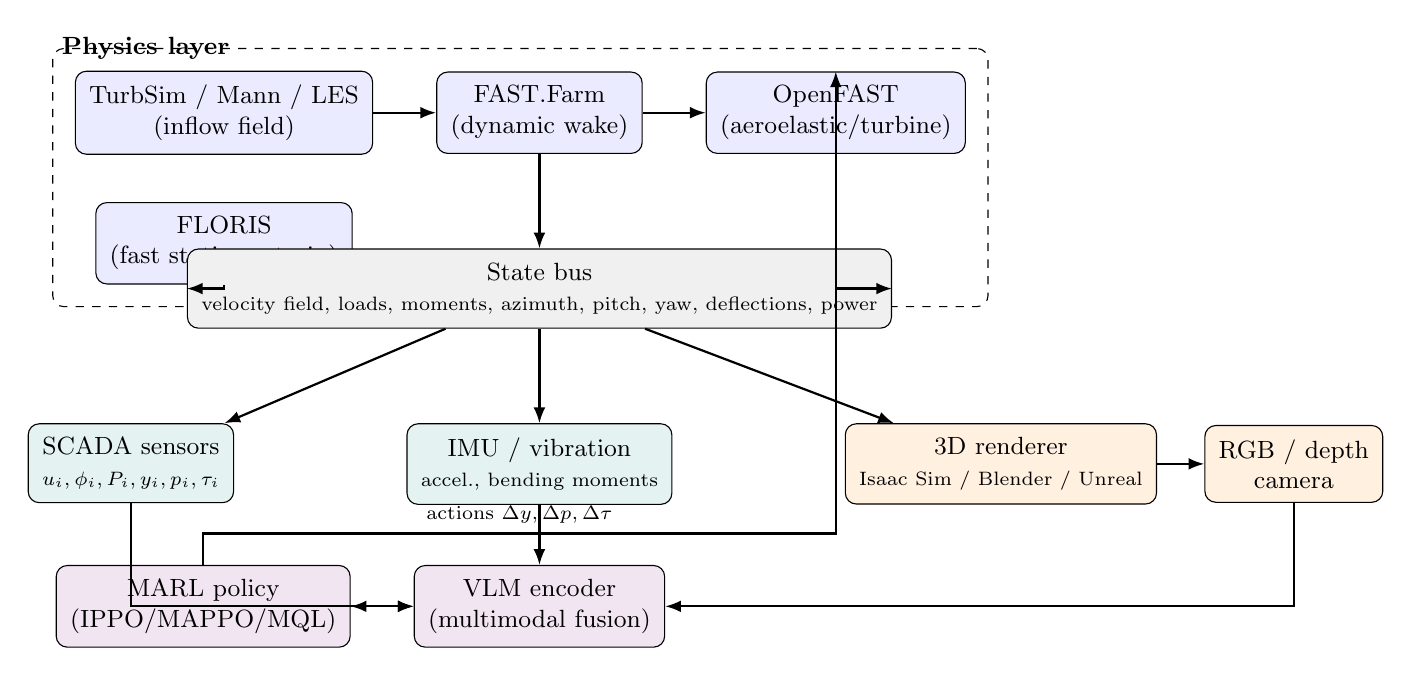
\begin{tikzpicture}[
  font=\small,
  box/.style={draw,rounded corners,align=center,inner sep=5pt,minimum height=9mm},
  phys/.style={box,fill=blue!8},
  sens/.style={box,fill=teal!10},
  render/.style={box,fill=orange!12},
  agent/.style={box,fill=violet!10},
  arr/.style={-{Latex[length=2mm]},thick},
  darr/.style={{Latex[length=2mm]}-{Latex[length=2mm]},thick}
]
% physics layer
\node[phys] (turbsim) {TurbSim / Mann / LES\\(inflow field)};
\node[phys,right=8mm of turbsim] (fastfarm) {FAST.Farm\\(dynamic wake)};
\node[phys,right=8mm of fastfarm] (openfast) {OpenFAST\\(aeroelastic/turbine)};
\node[phys,below=6mm of turbsim] (floris) {FLORIS\\(fast static pretrain)};

\begin{scope}[on background layer]
\node[draw,dashed,rounded corners,fit=(turbsim)(fastfarm)(openfast)(floris),
      inner sep=8pt,label={[anchor=west]north west:\textbf{Physics layer}}] (physlayer) {};
\end{scope}

% state bus
\node[box,fill=gray!12,below=12mm of fastfarm] (bus) {State bus\\
  {\scriptsize velocity field, loads, moments, azimuth, pitch, yaw, deflections, power}};

% sensor synthesis
\node[sens,below left=12mm and -6mm of bus] (scada) {SCADA sensors\\
  {\scriptsize $u_i,\phi_i,P_i,y_i,p_i,\tau_i$}};
\node[sens,below=12mm of bus] (imu) {IMU / vibration\\
  {\scriptsize accel., bending moments}};
\node[render,below right=12mm and -6mm of bus] (cam) {3D renderer\\
  {\scriptsize Isaac Sim / Blender / Unreal}};
\node[render,right=6mm of cam] (camout) {RGB / depth\\camera};

% agent
\node[agent,below=30mm of bus] (vlm) {VLM encoder\\(multimodal fusion)};
\node[agent,left=8mm of vlm] (policy) {MARL policy\\(IPPO/MAPPO/MQL)};

% arrows
\draw[arr] (turbsim) -- (fastfarm);
\draw[arr] (fastfarm) -- (openfast);
\draw[arr] (floris.south) |- (bus.west);
\draw[arr] (fastfarm) -- (bus);
\draw[arr] (openfast.south) |- (bus.east);
\draw[arr] (bus) -- (scada);
\draw[arr] (bus) -- (imu);
\draw[arr] (bus) -- (cam);
\draw[arr] (cam) -- (camout);
\draw[arr] (scada.south) |- (vlm.west);
\draw[arr] (imu) -- (vlm);
\draw[arr] (camout.south) |- (vlm.east);
\draw[darr] (vlm) -- (policy);
\draw[arr] (policy.north) -- ++(0,4mm) -| node[pos=0.25,above]{\scriptsize actions $\Delta y,\Delta p,\Delta\tau$} (openfast.north);
\end{tikzpicture}
\caption{Proposed co-simulation digital twin. The validated physics layer
(blue) is unchanged; sensor synthesis (teal) and rendering (orange) are added
around a shared state bus; a VLM fuses the modalities into observations for a
MARL policy that writes back control increments. FLORIS serves as a fast
static environment for pretraining/transfer.}
\label{fig:arch}
\end{figure}

\paragraph{Recommended tooling.}
\begin{itemize}[leftmargin=1.4em,itemsep=1pt]
  \item \textbf{Physics}: OpenFAST + FAST.Farm (both open, Apache-2.0);
  inflow via TurbSim/Mann, or high-fidelity LES (e.g.\ SOWFA/AMR-Wind) for
  ground truth. Keep FLORIS for cheap large-scale RL pretraining, then transfer
  (the paper's Transfer Task).
  \item \textbf{Rendering \& synthetic sensors}: \emph{NVIDIA Isaac Sim /
  Omniverse} is the natural fit---it ingests USD assets and provides built-in
  \emph{camera, depth, LiDAR, and IMU} sensor models with physically-based
  rendering and domain randomization, so the camera \emph{and} an independent
  IMU can be generated in one engine. Alternatives: Blender (Python-scriptable,
  photoreal Cycles), Unreal Engine (AirSim-style), Gazebo (lighter).
  \item \textbf{RL/MARL glue}: reuse WFCRL's Gymnasium/PettingZoo interfaces so
  IPPO/MAPPO/QMIX (and MQL) drop in unchanged; the VLM becomes a
  (frozen-or-fine-tuned) multimodal encoder in front of the policy/critic.
\end{itemize}

\paragraph{Where a Vision--Language model adds value.} Four concrete roles:
\begin{enumerate}[leftmargin=1.5em,itemsep=1pt]
  \item \textbf{Perceptual state augmentation}: detect visually-apparent
  conditions the SCADA vector misses---visible wake meander, icing, blade
  damage, smoke/fire---and fold them into the observation $o^i$.
  \item \textbf{High-level planner / coordinator}: a VLM reasons over the farm
  ``scene graph'' (the wake DAG of \S\,\ref{thm:networkmql}) and proposes
  yaw-steering intents that a low-level MARL policy executes.
  \item \textbf{Language-conditioned reward / preference model}: set the
  power--fatigue trade-off $\alpha$ in \eqref{eq:combined} or the weights
  $\rho_j$ in \eqref{eq:score} from natural-language operator goals (e.g.\
  ``prioritize blade life on the front row today'').
  \item \textbf{Inspection agent}: a maintenance VLM consuming rendered
  camera + vibration spectra to flag turbines for service---closing the loop
  from control to O\&M.
\end{enumerate}

\subsection{Honest limitations}

\begin{itemize}[leftmargin=1.4em,itemsep=1pt]
  \item \textbf{No free camera.} FLORIS/FAST.Farm give physics, \emph{not}
  pixels. Every visual claim rests on the fidelity of your renderer and its
  domain randomization; sim-to-real for RGB is a research problem in itself.
  \item \textbf{Dynamic-sim cost.} FAST.Farm is slow (the paper trains for
  \emph{days--weeks}); coupling a renderer per frame worsens throughput. Use
  FLORIS pretraining + FAST.Farm fine-tuning, and render only when the VLM is
  actually queried.
  \item \textbf{Validation envelope.} FAST.Farm power matches field data within
  $2$--$7\%$ (up to $18\%$ downstream at low wind); loads within $10\%$
  (up to $25\%$ for some directions). Vibration channels inherit these errors,
  so treat synthesized IMU data as \emph{plausible}, not calibrated, until
  validated against real turbine telemetry.
  \item \textbf{Theory scope.} The convergence guarantees of \cite{P2} assume
  a \emph{direct} observation of the exogenous inflow $w_\infty$ (transition
  independence) and \emph{finite} state/action tables. Rich pixel/vibration
  observations and function approximation (deep nets, VLMs) break both
  assumptions---extending the multi-scale guarantee to that setting is open
  (the authors flag ``noisy local observations'' and ``non-independent
  transitions'' as future work).
\end{itemize}

% =====================================================================
\section{Synthesis and research directions}
% =====================================================================

\begin{enumerate}[leftmargin=1.5em,itemsep=3pt]
  \item \textbf{Use WFCRL as the RL substrate, FAST.Farm/OpenFAST as the
  physics core, and add a renderer for vision.} This gives you all four sensor
  modalities you named; only the camera needs new engineering, and FAST.Farm
  already emits the kinematics to drive it.

  \item \textbf{Exploit the wake DAG in the learning architecture, not just the
  analysis.} The DAG of \S\,\ref{thm:networkmql} is a natural
  \emph{graph-attention} prior for a MARL critic or for a VLM's scene-graph
  reasoning; the multi-scale learning-rate assignment (Alg.~\ref{alg:lr}) is a
  ready-made curriculum/credit-assignment schedule.

  \item \textbf{Transfer is the crux.} Both papers stress that policies learned
  on static/low-fidelity models degrade on dynamic/real ones. A multimodal VLM
  encoder is attractive precisely because vision/vibration features may
  \emph{transfer} better than hand-picked SCADA scalars---worth testing as a
  sim-to-real robustness hypothesis.

  \item \textbf{Bring your stochastic-optimization toolkit.} The multi-timescale
  SA analysis (\S\,\ref{sec:sabackbone}) is directly your wheelhouse:
  two-/multi-timescale actor--critic convergence, Markovian-noise SGD, and
  ODE-method arguments all transfer. A concrete open problem: prove a
  multi-scale convergence result for \emph{function-approximation} MQL (linear,
  then deep), i.e.\ replace the tabular $Q^i$ with $Q^i_\theta$ and re-derive
  \eqref{eq:betacond} under a feature-space contraction.
\end{enumerate}

% =====================================================================
\begin{thebibliography}{9}
\bibitem{P1} C.~Bizon Monroc, A.~Bu\v{s}i\'c, D.~Dubuc, J.~Zhu.
  \emph{WFCRL: A Multi-Agent Reinforcement Learning Benchmark for Wind Farm
  Control.} NeurIPS 2024, Track on Datasets and Benchmarks.
\bibitem{P2} C.~Bizon Monroc, A.~Bu\v{s}i\'c, D.~Dubuc, J.~Zhu.
  \emph{Wind farm control with cooperative multi-agent reinforcement learning.}
  Workshop on Aligning RL Experimentalists and Theorists (ARLET), 2024.
\bibitem{borkar} V.~S.~Borkar. \emph{Stochastic approximation with two time
  scales.} Systems \& Control Letters 29(5):291--294, 1997.
\bibitem{kushneryin} H.~J.~Kushner, G.~G.~Yin. \emph{Stochastic Approximation
  and Recursive Algorithms and Applications.} Springer, 2003.
\bibitem{ppo} J.~Schulman, F.~Wolski, P.~Dhariwal, A.~Radford, O.~Klimov.
  \emph{Proximal Policy Optimization Algorithms.} arXiv:1707.06347, 2017.
\end{thebibliography}

\end{document}
